\documentclass{iopart}
\usepackage{iopams}
\expandafter\let\csname equation*\endcsname\relax
\expandafter\let\csname endequation*\endcsname\relax

%craft note: i had to remove this to get the citations working:
%\usepackage{harvard}

%\documentclass[12pt]{article}

% Misc. packages
\usepackage{appendix}
\usepackage{fancyvrb}
\usepackage{url}
\usepackage{hyperref}
\usepackage{authblk}
\usepackage{geometry}
\usepackage{enumerate}
\usepackage{lineno}

% Math & Symbol packages
\usepackage{mathtools,bm}
\usepackage{amsmath,amsfonts,amssymb}   %% AMS mathematics macros
\usepackage{amsmath}
\usepackage{amssymb}

% Graphics & Float packages
\usepackage{float}
\usepackage{graphicx}
%\usepackage{subfigure}
\usepackage{tikz}
\usepackage{pgfplots}
\pgfplotsset{compat=newest}

% Tikz and pgfplots libraries
\usetikzlibrary{patterns, arrows.meta, calc}
\usepgfplotslibrary{fillbetween}

% Colors
\usepackage{xcolor}
\definecolor{lightblue}{rgb}{0.0,0.5,0.8}
\definecolor{HMSRed}{HTML}{C5112E}  % [197, 17, 46]
\definecolor{MGHBlue}{HTML}{008BB0} % [0, 139, 176]
\definecolor{MGHGrey}{HTML}{626365} % [98, 99, 101]

% Annotation commands
\newcommand{\todo}[1]{{\color{lightblue}\par {[{\bf TO DO: } {\em #1}} ] \\    }}
\newcommand{\addref}[1]{{\color{red}{\bf [REF #1]}}}
\newcommand{\MPKcomment}[1]{{\color{magenta}\par {[{\bf MPK: } { #1}} ] \\    }}
\newcommand{\DCcomment}[1]{{\color{magenta}\par {[{\bf DC: } { #1}} ] \\    }}
\newcommand{\KvAcomment}[1]{{\color{magenta}\par {[{\bf KvA: } { #1}} ] \\    }}
\newcommand{\quotes}[1]{``#1''}   % Quotes!

% Document formatting
\linespread{1.4}
\geometry{
a4paper,
total={174mm,257mm},
left=20mm,
top=20mm,
}
\renewcommand{\floatpagefraction}{.8}
\renewcommand\Affilfont{\fontsize{9}{10.8}\itshape}

% This line prints line numbers
\linenumbers

%\renewcommand{\harvardurl}{URL: \url}

\begin{document}

\title[Dynamic MLC sequencing with splines ]{Solving the dynamic fluence map sequencing problem using piecewise linear leaf position and dose rate functions}
\author{Matthew Kelly, Koos van Amerongen,$^1$, David Craft$^2$}
\address{$^1$ Department of Econometrics and Operations Research/Center for Economic Research (CentER), Tilburg University, PO Box 90153, 5
000 LE Tilburg, The Netherlands}
\address{$^2$ Department of Radiation Oncology, Massachusetts General Hospital and Harvard Medical School, Boston, MA 02114, USA}
\ead{dcraft@mgh.harvard.edu}

\begin{abstract}
  Within the setting of intensity modulated radiation therapy (IMRT), and the fully continuous version of IMRT called volumetric modulated radiation therapy (VMAT), we consider the problem of matching a given fluence map as well as possible in limited time by the use of a multi-leaf collimator (MLC). We introduce two modeling strategies to manage the nonconvexity and the associated local minima of this problem. The first is the use of linear splines to model the MLC leaf positions and the dose rate as functions of time. The second is a progressively controllable smooth model (instead of a step function) of how the leaves block the fluence radiation. We solve the problem in two parts: an outer loop that optimizes the dose rate pattern over time, and an inner loop that, given a fixed dose rate pattern, optimizes the leaf trajectories.
\end{abstract}

\section{Introduction}
The optimal dynamic delivery of a given fluence map by a multi-leaf collimator (MLC) remains a difficult, largely unsolved problem.
The sliding-window leaf-sweep algorithm (SWLS) \cite{leafsweep},
    in which the MLC leaves cross the treatment field in a unidirectional fashion,
    achieves perfect fluence map replication if sufficient time is available \cite{Stein94}.
However, the SWLS algorithm is not in general efficient with respect to the required delivery time.
Time is an important aspect of VMAT and IMRT treatment plans, for several reasons:
\begin{enumerate}[i)]
  \item The effect of patient movement on delivery inaccuracy increases in the time the patient is exposed to radiation.
  \item Shorter treatments allow the treatment facility to help more patients on a given set of radiation therapy machines,
        which is particularly relevant to third-world countries as these machines are expensive.
  \item In general, there is a trade-off between dose quality and delivery time, and given how widespread the use of radiation therapy is in treating cancer, it makes sense to put in effort to assure that we are on the Pareto optimal frontier regarding these two objectives.

\end{enumerate}
Several studies have investigated the trade-off between treatment time and plan quality \cite{tradeoffSalari,tradeoffMCO,tradeoffCraft,balvertcraft}.
\cite{balvertcraft} were the first to include treatment time directly in a dynamic leaf sequencing step of the treatment plan optimization.
They constructed the trade-off curve between delivery time and fluence map matching accuracy by optimizing leaf trajectories and dose rate patterns for a sequence of delivery times.
% for several leaf trajectories independently
For a given fluence map and fixed delivery time, the challenge of optimizing the leaf trajectories and dose rate versus time so that the given fluence map is matched as accurately as possible, subject to machine restrictions, presents a high dimensional nonconvex optimization problem.
The nonconvexity of the fluence map matching problem leads to a large number of local minima.
For a thorough introduction to the complexities of dynamic fluence map delivery (which generally arises in the context of dynamic IMRT and VMAT),
 see \cite{balvertcraft} and \cite{unkvmatreview}.

\section{Methods}
\label{sec:model}

Our starting point is a fluence map $m$ that has been optimized, along with additional fluence maps located around the patient, to collectively yield a dose distribution optimized for the particular patient's geometry (location of tumor and all nearby organs) and dose prescription. We do not model this aspect of the problem and simply assume that the optimal fluence maps are given. The algorithms set forth in this paper determine how to construct a single given fluence map by moving the leaves of the MLC across the field, while varying the dose rate. Our optimization allows the leaves to move back and forth, a requirement for achieving optimal motions, as shown in the Appendix of \cite{balvertcraft}. Moreover, we allow the leaves of every pair to start and end separately and not necessarily at the bounds of the treatment field, as these restrictions can also be suboptimal \cite{thesisKvA}. Thus the problem we model and solve is the dynamic IMRT field delivery problem, which is a subproblem of the full dynamic VMAT problem \cite{vmerge}.

We assume the fluence map $m$ is given as a matrix where the rows correspond to the individual left and right leaf pairs, and the columns are the discretely optimized fluence bixels across the field, which can be as finely discretized as one wishes. Typical length scales are on the order of 0.5 cm for both the row height of the MLC leaves and the across-the-row discretization.

Let $x^i_L(t)$ and $x^i_R(t)$ denote the leaf position of the $i$th left and right leaves respectively, at time $t$. Our framework puts the dose rate optimization in an outer loop. Once the outer loop sets a dose rate over time profile, the leaf rows can be optimized independently (neglecting the small coupling terms created by the tongue-and-groove mechanism on the real machine, see \cite{unkvmatreview}), so for the remainder of the algorithm development, we consider only a single leaf row. Let $f(x)$ be the target fluence that should be delivered for that row. Note if $f$ is obtained from an optimized fluence map $m$ is is piecewise constant, but in general $f$ can also be smooth. We assume the total allowed treatment delivery time $T$ is given. Our goal is then to compute the dose rate $d(t)$ (outer loop) and the leaf trajectories $x_L(t)$ and $x_R(t)$ (inner loop) to recreate the fluence row $f(x)$ as best as possible, while accounting for maximum leaf speed, maximum dose rate, and collision constraints. We chose to focus on the leaf trajectory optimization in this report; the outer loop dose rate search is described in \ref{CMAES}.

The fluence achieved at each position is $g(x)$, which is the time-integral of the dose rate for the times that position is exposed to the radiation source.
The time domain of exposure $\mathcal{T}(x)$ is the set of times (in general a disconnected set) when the position $x$ is not blocked by either of the leaves, i.e.,
$\mathcal{T}(x)$ is the set of all times $t$ such that $x_L(t) \le x \leq x_R(t)$,
as illustrated by Figure \ref{fig:administeredDose} .

\begin{equation}
g(x) = \int_{t \in \mathcal{T}(x)} d(t) dt
\label{eqn:deliveredFluenceDose}
\end{equation}

Our goal is to find the leaf trajectories $x_L(t)$ and $x_R(t)$ and dose rate pattern $d(t)$
that minimize the squared integral error between the target fluence $f(x)$ and the delivered fluence $g(x)$:

\begin{equation}
\underset{d(t), \, x_L(t), \, x_R(t)}{\operatorname{argmin}}
\int_X \bigg(f(x) - g(x)\bigg)^2 dx .
\label{eqn:fluenceMapOptimization}
\end{equation}

% KvA: Example Figure, didn't care too much about efficiency
\begin{figure}[htp]
\centering
    \begin{tikzpicture}[remember picture]
        \pgfplotsset{holdot/.style={color=black,only marks,mark=*,mark size=1.5pt}}
        \pgfplotsset{soldot/.style={color=white,only marks,mark=*,mark size=1.5pt}}
        \begin{axis}[
            xmin=0, xmax=10.50,
            ymin=0, ymax=4.5,
            grid = both,
            grid style = dotted,
            axis x line = bottom,
            axis y line = left,
            enlargelimits = {abs=0.0},
            axis line style = {-Latex[round]},
            yticklabels = {$s$,$x$,$e$},
            ytick = {0.2,2,4},
            xtick = \empty,
            ylabel = {\scriptsize{position (cm)}},
            axis equal image
        ]

            % Vertical lines (top)
            \node[] (traj-1) at (axis cs:1,4.2) {};
            \node[] (traj-2) at (axis cs:1.88,4.2) {};
            \node[] (traj-3) at (axis cs:3.5,4.2) {};
            \node[] (traj-4) at (axis cs:4.17,4.2) {};
            \node[] (traj-5) at (axis cs:5.2,4.2) {};
            \node[] (traj-6) at (axis cs:5.85,4.2) {};
            \node[] (traj-10) at (axis cs:10,4.2) {};

            % Exposure times
            \draw[MGHBlue] (1,2) -- (1.89,2);
            \draw[MGHBlue] (3.5,2) -- (4.17,2.0);
            \draw[MGHBlue] (5.2,2) -- (5.85,2);

            % Leaf trajectories
            \addplot[name path global = leafl, black, smooth, tension=0.75] coordinates{(0,0.2)(1,2)(2.5,3.7)(4.7,1.9)(8.5,4)(10,4)};
            \addplot[name path global = leafr, black, smooth, tension=0.75] coordinates{(0,0.2)(1,0.5)(2.5,2.5)(4.5,1.4)(6.5,2.3)(8,2.1)(10,4)};

        \end{axis}
    \end{tikzpicture}

    \begin{tikzpicture}[remember picture]
        \pgfplotsset{holdot/.style={color=black,only marks,mark=*,mark size=1.5pt}}
        \pgfplotsset{soldot/.style={color=white,only marks,mark=*,mark size=1.5pt}}
        \begin{axis}[
            xmin=0, xmax=10.50,
            ymin=0, ymax=3.0,
            ymajorgrids = true,
            grid style = dotted,
            axis x line = bottom,
            axis y line = left,
            enlargelimits = {abs=0.0},
            axis line style = {-Latex[round]},
            xticklabels = {$T$},
            xtick = {10},
            yticklabels = {$d$},
            ytick = {2.5},
            xlabel style = {at={(ticklabel* cs:0.5,1.5)},anchor=north},
            xlabel = {\scriptsize{time(s)}},
            ylabel = {\scriptsize{dose rate (MU/s)}},
            axis equal image
        ]

            % Vertical lines (bottom)
            \node[] (dose-1) at (axis cs:1,-0.2) {};
            \node[] (dose-2) at (axis cs:1.88,-0.2) {};
            \node[] (dose-3) at (axis cs:3.5,-0.2) {};
            \node[] (dose-4) at (axis cs:4.17,-0.2) {};
            \node[] (dose-5) at (axis cs:5.2,-0.2) {};
            \node[] (dose-6) at (axis cs:5.85,-0.2) {};
            \node[] (dose-10) at (axis cs:10,-0.2) {};

            % Dose rate pattern
            \addplot[name path global = dose, black, smooth, tension=0.75] coordinates{(0,1.25)(2.5,2.4)(6,0.4)(8,1.9)(10,1.7)};\
            \addplot[name path global = xaxis, draw=none, domain=0:11] {0};

            % Integrals
            \addplot [thick, color=blue, fill=MGHGrey, fill opacity=0.2]
                fill between[of=xaxis and dose, soft clip={domain=1:1.88}];
            \addplot [thick, color=blue, fill=MGHGrey, fill opacity=0.2]
                fill between[of=xaxis and dose, soft clip={domain=3.5:4.17}];
            \addplot [thick, color=blue, fill=MGHGrey, fill opacity=0.2]
                fill between[of=dose and xaxis, soft clip={domain=5.2:5.85}];

            % Correction
            \addplot[fill = white]
                fill between[of=xaxis and dose, soft clip={domain=1.88:2}]; % filling
            \addplot[fill = white]
                fill between[of=xaxis and dose, soft clip={domain=4.17:4.5}]; % filling
            \addplot[fill = white]
                fill between[of=xaxis and dose, soft clip={domain=5.85:6}]; % filling
             \draw[black] (0,0) -- (10,0);

        \end{axis}
    \end{tikzpicture}

    \begin{tikzpicture}[remember picture,overlay]
        \draw[dashed,MGHGrey!60] (traj-1) -- (dose-1);
        \draw[dashed,MGHGrey!60] (traj-2) -- (dose-2);
        \draw[dashed,MGHGrey!60] (traj-3) -- (dose-3);
        \draw[dashed,MGHGrey!60] (traj-4) -- (dose-4);
        \draw[dashed,MGHGrey!60] (traj-5) -- (dose-5);
        \draw[dashed,MGHGrey!60] (traj-6) -- (dose-6);
        \draw[dashed,MGHGrey!60] (traj-10) -- (dose-10);
    \end{tikzpicture}

\vspace{-0.7cm}
\caption[Illustration of administered dose]{
    Illustration of administered dose: the dose administered to a position $x$ equals the integral (shaded area) of the dose rate (lower panel) over the moments in time (blue lines) that position is exposed by the leaves (upper panel).
    }
\label{fig:administeredDose}
\end{figure}


%\subsection{Scope of this work}

%-- Talk about how we limit scope of main paper to the leaf-trajectory optimization
%-- briefly discuss why we made this simplification, and how these results might be extended.

Next we describe the method that we use to convert this mathematical optimization problem into a format that can be solved using standard nonlinear programming (NLP) solvers such as FMINCON \cite{MatlabOptimizationToolbox2014}, SNOPT \cite{Snopt7}, or IPOPT \cite{Wachter2006}.

The first step in this process is to select a discrete representation for the leaf and dose rate trajectories, for which we use piecewise linear functions. The second step is to compute the integrals in the objective function using methods that are smooth and consistent, a critical step for obtaining good results from the NLP solver.

\subsection{Spline Representation}

There are three continuous functions that must be computed by the optimization: the position of the left and right leaves, $x_L(t)$ and $x_R(t)$, and the dose rate $d(t)$. We use piecewise linear functions (linear splines) to represent each function. A linear spline is fully defined by its value at the knot points $t_k$: $x_{L,k}$, $x_{R,k}$, and $d_k$. For simplicity we choose to use the same set of knot points for all three splines. An example of a linear spline is shown in Figure \ref{fig:linearSpline}.

\begin{figure}
  \centering
  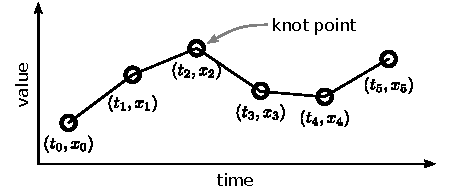
\includegraphics{fig/linearSpline.pdf}
  \caption{Linear Spline. We represent the dose rate and leaf position trajectories as linear splines. A linear spline is fully defined by its values at the knot points. }
  \label{fig:linearSpline}
\end{figure}

\subsection{Integral Computation with Blocking Function k()}
\label{sec:IntegralComputationWithBlockingFunction}

There are two issues with computing the integral in Equation \ref{eqn:fluenceMapOptimization} directly: 1) computing the domain $\mathcal{T}(x)$ requires a root solve (or inverting the leaf trajectories), and 2) the domain of $\mathcal{T}(x)$ can change from being simply connected to discontinuous during an optimization. Both of these issues would likely cause convergence failures in the NLP solver, in part by causing a change in the sparsity pattern of the gradient
(\textit{e.g.} $\tfrac{\partial g}{\partial x_L})$)
between successive iterations.

Our solution is to rewrite the integral using a blocking function $k(t,x)$, which has a value of one when the leaves at time $t$ are passing radiation at location $x$ and zero when the leaves are blocking radiation. This allows us to rewrite the integral using the constant bounds $[0, T]$:

\begin{equation}
  g(x) = \int_{t=0}^T \! k(t, x) \cdot d(t) \, dt
  \label{eqn:fluenceDoseSimpleBounds}
\end{equation}

We now have a standard scalar integral and we can use any quadrature method to evaluate (\ref{eqn:fluenceDoseSimpleBounds}).
In our case we use the midpoint (rectangle) quadrature rule.

As just defined, our fluence blocking function $k(t,x)$
would also have a discontinuous gradient, which would cause convergence issues in the optimization.
Therefore, we use an exponential sigmoid function 
to approximate the step function, where $\alpha$ is the smoothing parameter. 
\begin{equation}
  s(x, \alpha) = (1 + e^{-\alpha x})^{-1}
  \label{eqn:sigmoidEquation}
\end{equation}
A small value of alpha corresponds to heavy smoothing and faster convergence in the optimization, while a large value of alpha will provide a more accurate model at the expense of a more difficult optimization.
We can then combine the smoothing function for each leaf to get the combined blocking function:
\begin{equation}
  k(t, x) \approx \sqrt{s\big(x_R(t) -x, \, \alpha\big) \; \cdot \; s\big(x -x_L(t), \, \alpha\big)}
  \label{eqn:blockingFunction}
\end{equation}
\noindent In practice it is useful to define the $\alpha$ parameter in terms of 
a smoothing distance $\Delta x$ and 
the fraction $\gamma$ that the blocking function changed over that distance.
For example, $\Delta x = 0.05$ cm and $\gamma = 0.98$ means that 
the blocking function changes from $0.01$ to $0.99$ over a distance of $0.05$ cm.


\begin{equation}
  \alpha = \frac{-2}{\Delta x} \; \ln \! \left( \frac{1 - \gamma}{1 + \gamma} \right)
  \label{eqn:SmoothingDistanceParameter}
\end{equation}

Figure \ref{fig:visualizeExponentialSmoothing} shows three values of the smoothing parameter for the blocking function $k(t, x)$, where $x_R = 1$ and $x_L = -1$, and compares the function to the case without smoothing.

\begin{figure}
  \centering
  \includegraphics[width=\textwidth]{fig/FIG_visualize_exponential_smoothing.pdf}
  \caption{Visualization of smoothing parameters in the blocking function (\ref{eqn:blockingFunction}. The right and left leaves are at $x_R = 1$ cm and $x_L = -1$ cm respectively. The solid black line shows the case without smoothing, and the remaining lines show light smoothing ($\Delta = 0.05$ cm), moderate smoothing ($\Delta = 0.2$ cm), and heavy smoothing $\Delta = 0.5$ cm). In each of these three cases we use a value of $\gamma = 0.95$.}
  \label{fig:visualizeExponentialSmoothing}
\end{figure}

%\subsection{Objective Function}

The objective function for the inner optimization (computing leaf trajectories)
is the integral of the error-squared between the desired fluence $f(x)$ and the fluence that
is delivered by the current set of trajectories, $g(x)$.
\begin{equation}
  J = \int_{x_\text{min}}^{x_\text{max}} \! \bigg( f(x) - g(x) \bigg)^2 \,dx
  \label{eqn:continuousFittingObjective}
\end{equation}

In practice we can only compute the fluence profile at a finite number of points. We will break the domain $[x_\text{min}, x_\text{max}]$ into $N_\text{fit}$ equal-width segments,
and evaluate the fluence target and delivered fluence at the midpoint $x_k$ of each segment.

\begin{equation}
  J \approx \frac{x_\text{max} - x_\text{min}}{N_\text{fit}}
  \sum_{k = 1}^{N_\text{fit}} \! \bigg( f(x_k) - g(x_k) \bigg)^2
  \label{eqn:discreteFittingObjective}
\end{equation}

\subsection{Computing Leaf Trajectories as a Nonlinear Program}
\label{sec:LeafTrajectoryAsNLP}

The inner optimization loop computes the leaf trajectories $x_L(t)$ and $x_R(t)$
that minimize the objective function (\ref{eqn:discreteFittingObjective})
and satisfy the position and velocity constraints given below.
This optimization is solved as a nonlinear program.

We model the leaf trajectories as piecewise-linear functions of time,
where the decision variables in the optimization are the position of each leaf
at the knot points in the spline: $x_{L, k}$, $x_{L, k}$, as shown in Figure \ref{fig:linearSpline}. We compute the position on each segment by linear interpolation between the knot points. The velocity of the leaf on each segment is constant and is given by:
\begin{equation}
  \dot{x}_{L, k} = \frac{x_{L, k+1} - x_{L, k}}{h_k}
  \quad \quad
  \dot{x}_{R, k} = \frac{x_{R, k+1} - x_{R, k}}{h_k}
\end{equation}
\noindent where $h_k$ is the distance between knot point $k$ and $k+1$ (we use equal spacing for all knot points).

The limits on leaf position can be implemented as a combination of
constant bounds and linear inequality constraints:

\begin{equation}
  x_\text{min} \leq x_{L, k}
  \quad \quad
  x_{R, k} \leq x_\text{max}
  \quad \quad
  x_{L, k} \leq x_{R, k}
  \quad \quad
  \forall k
  \label{eqn:PositionLimits}
\end{equation}

The limits on velocity can be written as linear inequality constraints:

\begin{equation}
  -v_\text{max} \leq \dot{x}_{L, k} \leq v_\text{max}
  \quad \quad
  -v_\text{max} \leq \dot{x}_{R, k} \leq v_\text{max}
  \quad \quad \forall k
  \label{eqn:VelocityLimits}
\end{equation}

At this point we can compute the piecewise-linear position trajectories and the
piecewise-constant velocity trajectories, and enforce limits on them inside the non-linear program.
The final step is to compute the objective function for the candidate trajectories,
which is done as described in Section \S~\ref{sec:IntegralComputationWithBlockingFunction}.

\subsection{Iterative refinement of smoothing parameter}

The performance of the optimization, based on solve-time and accuracy, is highly dependent on the value of the smoothing parameter $\alpha$. With heavy smoothing the optimization will quickly converge to a \quotes{good} solution, but the smoothing distorts the objective function to the point where it is innacurate. Conversely, with light smoothing (or no smoothing) the gradients in the optimization change quickly and the solver easily gets stuck in local minima and sometimes fails to converge.

This dependency on smoothing is common in trajectory optimization, and there is a well known solution: iterative refinement. The idea is to initially solve the optimization using heavy smoothing, which gives a solution that is somewhat close to the true optimal solution. Then the optimization is solved again, using the previous solution as the initial guess and with a smaller value of the smoothing parameter. This process is continued until the error in the objective function decreases to an acceptable level \cite{Srinivasan2006}.

\section{Results}

\subsection{Smoothing Parameter iteration schedule}

One of the key parameters in the optimization is the smoothing parameter $\alpha$, which we compute here using equation (\ref{eqn:SmoothingDistanceParameter}), using a characteristic smoothing width $\Delta x$ and a parameter $\gamma$ that describes how much the blocking function changes over that smoothing width. 

For this experiment we set a constant $\gamma = 0.95$ and then study three values for the ``smoothing distance'' $\Delta x = \{0.5, 0.2, 0.05\}$ cm. We compute the optimal leaf trajectory pair for two example fluence profiles, one with a unimodal structure and one with a bimodal structure (see Figures \ref{fig:smoothingParamSweep_unimodalTraj} and \ref{fig:smoothingParamSweep_bimodalTraj}). In each case we use $n=6$ grid points on the leaf trajectories.

We explore each possible sequence of smoothing iterations for these three parameters. In general, it would be possible to automate this refinement, but simply starting heavy smoothing and then decreasing the smoothing on successive iterations until a desired accuracy is achieved.

\begin{figure}
  \centering
  \includegraphics[width=\textwidth]{fig/FIG_smoothingParamSweep_pareto.pdf}
  \caption{Comparison of the optimization for two different fluence profiles (See Figures \ref{fig:smoothingParamSweep_unimodalTraj} and \ref{fig:smoothingParamSweep_bimodalTraj}) for a variety of smoothing parameter iteration schedules. The resulting solutions are evaluated based on CPU time and objective value: fitting error computed without smoothing.}
  \label{fig:smoothingParamSweep_pareto}
\end{figure}


\subsection{Leaf trajectory plots for two examples}

In the previous section we showed a comparison of the objective function values for various smoothing schedule. Here we select a single smoothing schedule ($\Delta = 0.5 \to 0.2$) and show the optimal leaf trajectories for both the unimodal and bimodal examples.

\begin{figure}
  \centering
  \includegraphics[width=\textwidth]{fig/FIG_smoothingParamSweep_unimodalTraj.pdf}
  \caption{The optimal leaf trajectories for the unimodal example problem, computed using the smoothing schedule ($\Delta = 0.5 \to 0.2$). The right plot shows the leaf trajectories, and the left plot shows the target and delivered fluence for a constant dose rate.}
  \label{fig:smoothingParamSweep_unimodalTraj}
\end{figure}


\begin{figure}
  \centering
  \includegraphics[width=\textwidth]{fig/FIG_smoothingParamSweep_bimodalTraj.pdf}
  \caption{The optimal leaf trajectories for the bimodal example problem, computed using the smoothing schedule ($\Delta = 0.5 \to 0.2$). The right plot shows the leaf trajectories, and the left plot shows the target and delivered fluence for a constant dose rate.}
  \label{fig:smoothingParamSweep_bimodalTraj}
\end{figure}

\subsection{Objective function value during the optimization}
\begin{figure}
  \centering
  \includegraphics[width=\textwidth]{fig/CPUvsObj_Pr-2-row11-bi_Smooth-05-02.pdf}
  \caption{Relation between CPU time and the best known smoothed objective value and the corresponding exact objective value, for the parameter scheme ($\Delta x= 0.5 \to 0.2$) and the unimodal fluence profile (see Figure \ref{fig:smoothingParamSweep_unimodalTraj})}
  \label{fig:CPUvsObj_bestalpha_uni}
\end{figure}

\subsection{Objective function value during the optimization}
\begin{figure}
  \centering
  \includegraphics[width=\textwidth]{fig/CPUvsObj_Pr-2-row11-bi_Smooth-05-02.pdf}
  \caption{Relation between CPU time and the best known smoothed objective value and the corresponding exact objective value, for the parameter scheme ($\Delta x= 0.5 \to 0.2$) and the bimodal fluence profile (see Figure \ref{fig:smoothingParamSweep_bimodalTraj})}
  \label{fig:CPUvsObj_bestalpha_bi}
\end{figure}

\todo{All: finetune figures}
\todo{Koos: explain/interpret figures}

\section{Discussion and conclusions}

\subsection{Smoothing schedule}

The various smoothing schedules can be analyzed on a pareto front, with a trade-off between CPU time and the value of the objective function. Heavy smoothing (large $\Delta$) results in fast optimization but poor fitting. Light smoothing results in slow optimization as well as poor fitting. The best solutions were obtained by starting with heavy smoothing and then moving to moderate smoothing. These solutions required a moderate amount of CPU time but tended to be more accurate than other methods.

\subsection{Smoothed vs Exact objective function}

In all of the optimizations we used a smooth objective function for the optimization, but also track the performance of the ``true'' objective function (no smoothing). For heavy smoothing there is a significant difference between the two, but with light smoothing the difference is negligible.

\todo{Koos: discuss your plot for obj. val. vs time here?}
\KvAcomment{Matthew: I think these plots better fit in the previous section. We could directly discuss the figures there.}

\subsection{Fitting performance}

For simple fluence target profiles we were typically able to obtain the desired fluence profile to within the accuracy of our model. For more complex profiles, such as the bimodel profile shown in the figure \ref{fig:smoothingParamSweep_bimodalTraj}, the fluence target was matched reasonably well, with some small fitting errors near sharp changes in the profile. These errors are in part due to using a small number of linear segments to represetn the leaf trajectories.

\subsection{Choice of grid-point count}

All of the experiments in this report used six grid-points (five segments) for the leaf trajectories. This number was chosen using a pilot study. If fewer grid-points were used, then the ability to fit arbitrary profiles was diminished. If more grid-points were used then there was a minor improvement in fitting, but a significant increase in computational time and it was more difficult to find a viable smoothing schedule.

\subsection{monotonic vs non-monotonic leaf trajectories.}

\todo{David: thoughts on discussing non-montonic leaf trajectories?}


\subsection{How long should the duration of the trajectory be?}

The duration of the trajectory is another important parameter when computing the optimal set of leaf trajectories. For this report we will consider it fixed, assuming that it is computed by some outer optimization loop, along with the dose-rate trajectory.
\KvAcomment{Let's discuss several delivery times, at least in the appendix when also discussing the outer (dose rate space search) loop. Also, even then, we would have to manually pick values for $T$.}

\subsection{Why first-order splines to represent trajectories?}
\label{sec:WhyUseLinearSplines}

There are many choices for representing trajectories, most of which can be classified as a type of polynomial spline. There is a fundamental trade-off in polynomial splines: for a given amount of data you can store many low-order segments or few high-order segments. Selecting the correct trade-off is discussed in detail in \cite{kelly2017introduction}, \cite{Betts2010}, \cite{Darby2011a}. 

In this paper we use a linear spline: many low-order segments rather than few high-order segments. One reason for this choice is that we can precisely enforce velocity constraints without the need for mesh refinement or other expensive checks. The low order spline also lends itself to fast and simple calculations. Finally, our model is not accurate enough to necessitate the complexity associated with higher-order methods.

We performed a brief pilot study, where we compared linear to cubic splines, with the same number of decision variables in the optimization. We found that the linear splines resulted in faster optimization for a comparable accuracy and dramatically simplified the resulting optimization code.


\section{Conclusions}

\todo{once we get the rest of the paper written}

\section{Future Work}

The next steps for this project are include this leaf-trajectory optimization as the inner loop in some larger optimization that computes the optimal dose rate and trajectory duration.

\todo{Add more detail here}


\appendix

\section{Comparison to Existing methods}

\todo{Koos  --  maybe put some of those fancy Tikz figures with the heat maps in here?}

\section{Computing dose rate trajectories and total time}
\label{CMAES}

\todo{Koos --  pull in old CMAES stuff?}

\bibliographystyle{unsrt}
\bibliography{all}

\end{document}
